\documentclass[11pt,letterpaper,twocolumn]{article}
\usepackage[utf8]{inputenc}
\usepackage[spanish]{babel}
\usepackage{amsmath}
\usepackage{amsfonts}
\usepackage{amssymb}
\usepackage{float}
\usepackage{graphicx}
\usepackage{listings}
%\usepackage{fourier}
\usepackage[left=2cm,right=2cm,top=2cm,bottom=2cm]{geometry}
%\author{miguel}
\begin{document}
%Simulación en Python de un tiro bidimensional en un contorno cerrado con dispersores en el centro, utilizando el método de Runge Kutta.\\
\title{\huge{\textbf{
Python simulation of a two-dimensional shot in a closed contour with dispersers in the center, using the Runge Kutta method.}}}
\author{\small \textit{M. Sabogal $^{1}$}\\
	\small \textit{ $^{1}$ Estudiante del programa de Física, Universidad del Atlántico, Barranquilla-Colombia}}
\date{} 

\twocolumn[
\begin{@twocolumnfalse}
\maketitle
\begin{center}
{\rule[0mm]{160mm}{0.2mm}}
\end{center}
\begin{abstract}
\textit{Se simuló el lanzamiento bidimensional de una partícula de masa $m$ en un entorno circular cerrado, con cuatro dispersores iguales situados en el centro, utilizando el lenguaje computacional de phyton y el runge kutta de orden 4, de manera que se describiera la trayectoria de la partícula a partir de las condiciones iniciales $(\vec{r_{o}}, \vec{v_{o}})$. Luego mediante los coeficientes de Lyapunov se comprobó que el sistema presenta caos, y se observo la región caótica para un set de parámetros específicos, también se demostró que el grado de dispersión de las partículas (ángulo de salida), depende del parámetro de impacto y de la energía inicial de lanzamiento, y de manera similar se determino la sección eficaz, a partir de la distribución de impacto sobre el contorno de la región circular.\\
\\
\textbf{Palabras claves: Dispersores,Caos, Runge Kutta, Lyapunov.}}
\begin{center}
\textbf{Abstract} 
\end{center}
\par 
\textit{it was simulated the bidimensional launching of a particle of mass $ m $ in a closed circular environment, with four equal dispersers located in the center, using the computational language of phyton and the runge kutta of order 4, to describe the trajectory of the particle from the initial conditions $ (\ vec {r_ {o}}, \ vec {v_ {o}}) $. Then, using the Lyapunov coefficients, it was observed that the system presents chaos, and the chaotic region was observed for a set of specific parameters. It was also shown that the degree of dispersion of the particles depends on the impact parameter and of the initial energy of launching, and in a similar way the effective section was determined, from the distribution of impact on the contour of the circular region.\\
\\
\textbf{Keywords: Dispersers, chaos, Runge Kutta, Lyapunov.}}
\end{abstract}
\begin{center}
{\rule[0mm]{160mm}{0.2mm}}
\end{center}
\end{@twocolumnfalse}
]

\section*{\normalsize{INTRODUCCIÓN}} 
El término “caos” (del griego \textit{$\chi\alpha o  \sigma$} : “abertura, oquedad insondable”) usualmente se refiere a los acontecimientos aparentemente aleatorios, es decir, los que ocurren sin un orden; este uso parecería ser inamovible, al menos a primera vista. Sin embargo, la teoría del caos se centra en la noción de que el análisis de lo aparentemente impredecible conduce al esclarecimiento de un orden. El caos es determinable, y no es aleatorio porque tiene un orden subyacente. Un proceso caótico puede parecer aleatorio (al azar, sin orden), pero el análisis total del proceso lleva a distinguir algunos episodios ordenados (que dejan de ser caóticos), entremezclados con otros aleatorios (de los que quizá sólo se desconocen, de momento, las reglas que establecen su causalidad).$^{[4]}$\\
\par 
Se desea estudiar, la manera como se ven afectadas una o mas partículas lanzadas en dos dimensiones hacia el centro de un entorno circular cerrado, con cuatro dispersores (potenciales repulsivos) situados en el centro de la zona de estudio, también se pretende encontrar la sección eficaz de impacto y la zona en la que se presenta mayor caos en función del parámetro de impacto.
\subsection*{Sistemas caoticos}
El concepto de caos es muy delicado, debido a que no existe una definición única. Sin embargo, mencionar la palabra caos trae inmediatamente algo a la mente: falta de orden o de capacidad de predicción. Cómo fue previamente mencionado el caos no implica aleatoriedad, un sistema en el que se presenta caos se denomina sistema caótico, éstos sistemas presentan algunos rangos importantes cómo:
\begin{enumerate}
\item El determinismo, es decir existe alguna regla matemática que describa el comportamiento del sistema. 
\item La sensibilidad a las condiciones iniciales, es decir, que aun con condiciones iniciales arbitrariamente cercanas, dos eventos tendrán comportamientos completamente distintos en el futuro. Una manera de cuantificar esta propiedad es mediante los coeficientes de Lyapunov. 
\end{enumerate}
\par 
%%Estas dos últimas propiedades son necesarias para tener caos, no basta tener solo sensibilidad a condiciones iniciales. Como ejemplo tomemos el sistema que consiste en doblar repetidamente un valor inicial. Este sistema tiene sensibilidad a condiciones iniciales, pues todo par de valores cercanos eventualmente se separarán tanto como uno quiera con el tiempo, de manera exponencial. Es evidente también que en este sistema tampoco hay caos.$^{[]}$ 
\subsubsection*{Coeficientes de Lyapunov}
Una de las principales herramientas en el estudio de los sistemas dinámicos son los coeficientes caracteristicos de Lyapunov; éstos miden la estabilidad o inestabilidad de las trayectorias del sistema bajo perturbaciones pequeñas, o lo que es lo mismo, la sensibilidad a las condiciones iniciales.\\
\par 
Consideremos un sistema dinámico diferenciable $^{[3]}$:
$$\dot{Z}=F(Z)$$
\par 
Donde $Z$ es un vector del espacio fase del sistema, que tiene dimensión $L$. Al integrar este conjunto de ecuaciones diferenciales acopladas obtenemos la evolución temporal del sistema, el llamado flujo en el espacio fase, dado por:
$$Z(t)=\Phi^{t}(Z(0))$$
\par
Donde $Z(t)$ es la solución al tiempo $t$. Tomemos una trayectoria de referencia $Z(t)$, y una trayectoria perturbada $Z_{s}(t)$ conectada con $Z(t)$ por una curva parametrizada con parámetro $s$ tal que, el vector tangente asociado es:
$$\delta Z(t)=\lim_{s \to 0}	 \dfrac{Z_{s}(t)-Z(t)}{s}$$
\par 
Su ecuación de movimiento se obtiene linealizando $\dot{Z}=F(Z)$:
$$\delta\dot{Z}=D(Z) \delta Z$$
\par 
Donde $D(Z)= \partial F(Z)/ \partial Z$ es la matriz jacobiana del sistema. Para sistemas caóticos, la perturbación $\delta Z(t)$ crece exponencialmente, lo que motiva la definición de los exponentes de Lyapunov de una trayectoria con condiciones iniciales $\delta Z(0)$ cómo:
$$\lambda (Z(0),\delta Z(0))= \lim_{t \to T} \log \dfrac{\vert \delta Z(t)\vert}{\vert \delta Z(0)\vert}$$
\par 
Ésta ecuación se puede reescribir como una estimación para el cambio de tamaño en la separación inicial cómo:
\begin{equation}
\vert \delta Z(t)\vert \approx \vert \delta Z(0)\vert e^{\lambda t}
\label{coef}
\end{equation}
\par 
De la cual se deduce que si $\vert \lambda \vert > 1$, la separación entre las trayectorias crecerá de manera exponencial, es decir son perturbaciones inestables (caóticas). Mientras que si $\vert \lambda \vert < 1$ se presenta estabilidad. 
\subsection*{Modelo mesa de billar}
Cómo modelo de estudio, se considera el lanzamiento en dos dimensiones de una partícula hacia el centro de un entorno circular cerrado (mesa de billar), con cuatro dispersores iguales (potenciales repulsivos) situados alrededor del centro de la mesa, donde el potencial de cada dispersor ésta dado por la expresión:\\
$$V_{i}(x,y)=A e^{-\alpha[ (x-x_{o_{i}})^{2} + (y-y_{o_{i}})^{2} ]}$$  
\par 
Donde $A$ es la amplitud del campo (valor máximo), el inverso de $\alpha$ determinará la extensión del potencial, y ($x_{o_{i}},y_{o_{i}}$) es la posición del centro del potencial. Recordando que para sistemas conservativos se tiene:
$$\vec{F_{i}}=- \vec{\nabla}V_{i}=- (\dfrac{\partial V_{i}}{\partial x},\dfrac{\partial V_{i}}{\partial y})$$ 
\par 
A partir de la segunda ley de newton y considerando que la partícula solo interactúa con los cuatro potenciales, se deduce una expresión para describir la aceleración total de la partícula durante su trayectoria:
$$\dfrac{d^{2}\vec{r_{i}}}{dt^{2}}=\dfrac{2 \alpha A}{m} e^{-\alpha[ (x-x_{o_{i}})^{2} + (y-y_{o_{i}})^{2} ]} [(x-x_{o_{i}}),(y-y_{o_{i}})]$$
\begin{equation}
\dfrac{d^{2}\vec{r}}{dt^{2}} = \sum_{i=1}^{i=4} \dfrac{d^{2}\vec{r_{i}}}{dt^{2}}
\label{aceleracion}
\end{equation}
\par 
La ecuación \ref{aceleracion} es una EDO de segundo orden que se debe resolver para tener pleno entendimiento del fenómeno, teniendo en consideración que en este caso la aceleración no depende explícitamente del tiempo sino de la posición de la partícula con respecto al centro de cada potencial y a los parámetros $A$,$m$ y $\alpha$.\\
\section*{-Interpretación física y resultados}
Con el fin de estudiar el movimiento de una partícula en dos dimensiones que es lanzada hacia el centro de una mesa de billar, con cuatro dispersores iguales situados alrededor del centro de la mesa, se simulo el \textbf{modelo mesa de billar}, utilizando el lenguaje de programación de python. En primera instancia se establece la localización del observador, colocando la referencia espacial $(0,0)$ en el punto central de la mesa, de radio R, y el tiempo cero justo al inicio del lanzamiento; la posiciones de los potenciales se establecen de manera que los cuatro se encuentren a la misma distancia del observador, y de igual forma sus centros coincidan con los vértices de un cuadrado con lados de longitud a, es decir los cuatro potenciales se encuentran en las coordenadas espaciales $(a,a)$,$(a,-a)$,$(-a,-a)$ y $(-a,a)$ respectivamente, y donde la aceleración que la partícula experimenta esta descrita por la ecuación \ref{aceleracion}. Este modelo se estudiará desde la perspectiva de los sistemas dinámicos, permitiendo describir la evolución del sistema a partir de la evolución de la velocidad y posición en función del tiempo, es decir encontrar un vector “Y” que contenga estas cantidades. Para lograr esto se sabe que la velocidad es la derivada temporal de la posición, y la aceleración es la derivada de la velocidad con respecto al tiempo, tomando el conjunto de estas cantidades como la derivada en el tiempo del vector dinámico$^{[1]}$ $Y$, se tiene:\\ 
$$ F(Y,t)=\dfrac{dY}{dt}=(\vec{v},\vec{a})=( \dfrac{dx}{dt},\dfrac{dy}{dt},\dfrac{dv_{x}}{dt},\dfrac{dv_{y}}{dt}) $$
\par 
Al integrar esta expresión con respecto al tiempo, se obtiene la manera de cómo evoluciona el sistema.\\
$$ Y_{n}= Y_{n-1} + \int_{t_{n-1}}^{t_{n}} F(Y,t)dt  $$
\par 
A través del runge kutta de orden 4, con paso estándar de $h=10^{-2}$, se calculó el vector dinámico para el lanzamiento de una partícula transcurrido un cierto tiempo, hasta que golpeara el contorno de la mesa, partiendo de unas condiciones iniciales dadas $(\vec{r_{o}},\vec{v_{o}})$; las cuales se establecieron de manera que la partícula fuera lanzada desde un punto con un valor en x, de $x_{o}$, a lo largo de la recta $y=-3R/4$, es decir $\vec{r_{o}}=(x_{o},-3R/4)$, y el vector velocidad inicial estuviera descrito por $\vec{v_{o}}=(v_{o}\cos\theta,v_{o}\sin\theta)$ , donde $v_{o}$ es la magnitud de la velocidad inicial y $\theta$ el ángulo de tiro; sin embargo, en la presente solución solo se considero el caso cuando el ángulo de tiro es $\theta=90 ^{\circ}$ con respecto a la horizontal, es decir que $\vec{v_{o}}=(0,v_{o})$.\\
\par 
Cómo fue previamente discutido, el movimiento de la particula no solo depende de las condiciones iniciales, sino de su interacción con los potenciales, a partir de ésta idea se estableció un set de parámetros en los cuales se define la masa $m$ de la particula, la amplitud $A$ (intensidad maxima) de los potenciales, $\alpha$, el radio $R$ de la mesa y las posiciones de los centros de cada potencial.\\
\par 
Posteriormente, se realizó un vector de condiciones iniciales de cuatro componentes, que consta de las posiciones y velocidades iniciales, desde el cual parte la integración del runge kutta, generando una matriz que representa el vector dinámico de la partícula, desde que es lanzada hasta que choca con el contorno de la mesa. Esto se condicionó en el rugen kutta de modo que se detuviera la integración cuando la suma de las componentes al cuadrado fuera mayor o igual que el radio al cuadrado $x^{2} + y^{2} \geq R^{2}$. Debido al paso del runge kuta y al condicional impuesto, la última posición de la partícula se encuentra por fuera del circulo, es decir de la mesa. Para corregir este error se implementó un condicional que recalculara a partir del penúltimo paso, nuevamente el ultimo, con un paso de $h_{2}=h/4$ con respecto al $h$ anterior, permitiendo obtener una buena aproximación del momento justo cuando choca con el contorno de la mesa.\\
\par
Se crearon dos clases, una llamada “Potencial” que almacenara la información relevante del dispersor en cuestión, y tuviera dos métodos que permitieran determinar el valor del potencial y la aceleración que una partícula de masa $m$ experimentaría por su interacción con él, en un punto del espacio; y la otra clase llamada “Partícula”, que guardara la información de la trayectoria y velocidades de una partícula luego de un lanzamiento, y que tuviera tres método que entregaran el ángulo de salida, el ángulo de impacto y las energías del sistema, a partir de un set de parámetros pre-establecidos.\\ 
\par 
En la figura \ref{f1}, se visualiza la trayectoria de una partícula de masa $m=1$ después de un lanzamiento desde $x_{o}=-0.7$, con velocidad inicial $v_{o}=1.60005$, con dispersores de amplitud $A=3$ y $\alpha=0.5$ en las posiciones correspondientes a $a=2$; en la que se puede apreciar la manera como es afectada su trayectoria producto de la interacción con los potenciales.\\ 

\begin{figure}[H]
\centering 
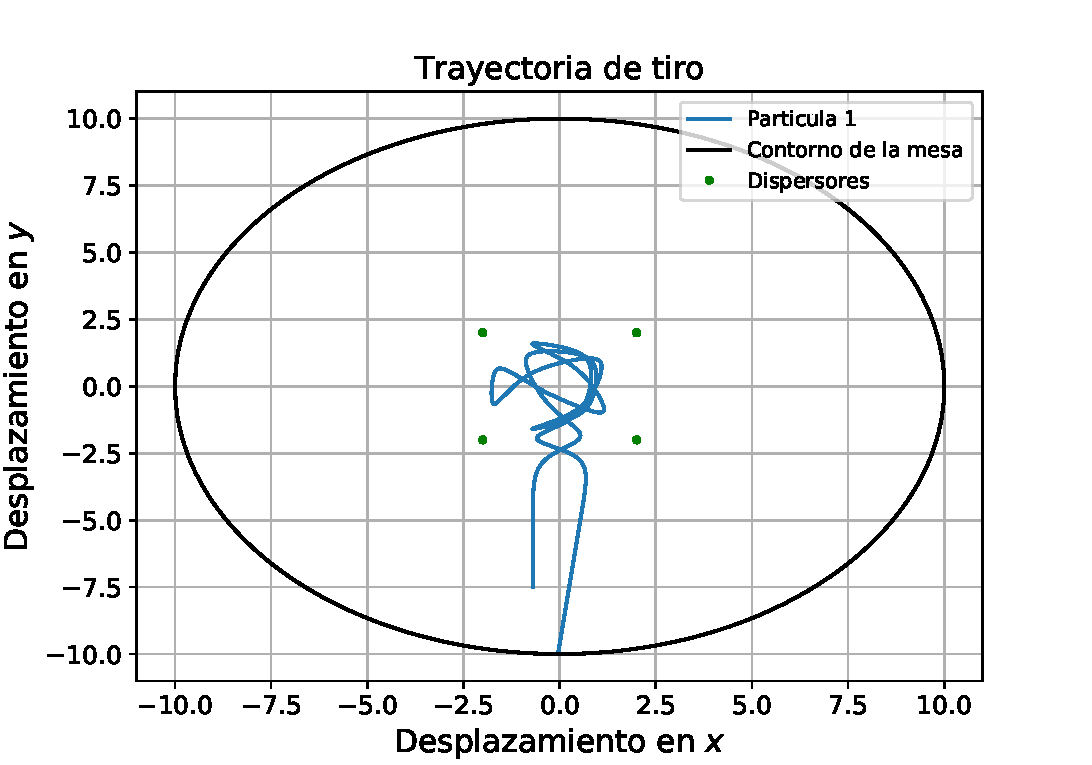
\includegraphics[scale=0.5]{g1.pdf}
\caption{Gráfica de la trayectoria 1 con parámetros=[m: 1, $\alpha: 0$.$5$, $R: 10$ , $A: 3$, $ x_{o}: -0$.$7$,$ v_{o}: $1.$60005$, $a$: 2]} 
\label{f1}
\end{figure}  

\par 
Se observa en la figura anterior, que durante un tiempo la partícula describe una trayectoria alrededor del centro de la mesa, que coincide con el centro común de los potenciales. Al ser éstos repulsivos y la manera como “orbita", la partícula alrededor de éste punto, sugiere la existencia de un pozo de potencial cómo se observa en la figura \ref{f2}, donde está representada la intensidad normalizada del campo (potencial) en un diagrama de colores; permitiendo visualizar de mejor manera la forma como interactúa la partícula con los potenciales y la geometría del pozo.\\
\begin{figure}[H]
\centering 
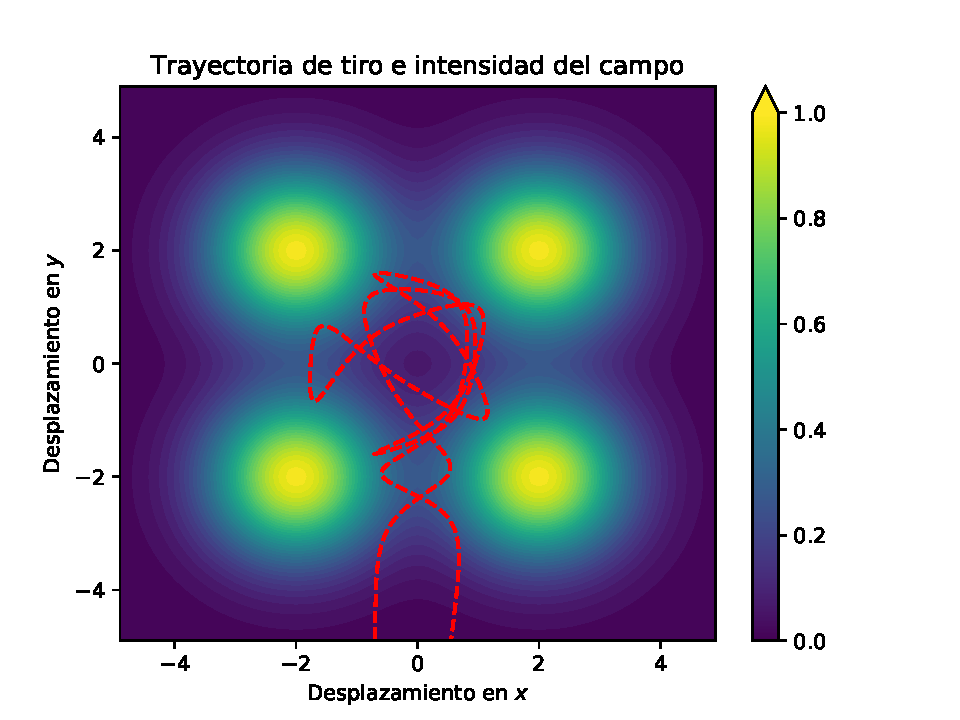
\includegraphics[scale=0.55]{g2.pdf}
\caption{Trayectoria 1 e intensidad del campo.}
\label{f2}
\end{figure}  
\par 
Ya que las fuerzas involucradas son conservativas, la energía del sistema se debe conservar, cómo se observa en la figura \ref{ene}, la cual presenta las energías del lanzamiento de la figura \ref{f1} en función del tiempo, y la energía total del sistema, la cual es una constante. De ésta figura también se observa la forma como los potenciales modifican la trayectoria de la partícula, al analizar los picos de la energía potencial que conllevan a mínimos de la energía cinética, se observan los instantes cuando la partícula es detenida por uno de los potenciales y es repelida en otra dirección; y para los máximos de la energía cinética, se observa como disminuye (mínimos de la energía potencial) la interacción con los dispersores.\\
\begin{figure}[H]
\centering 
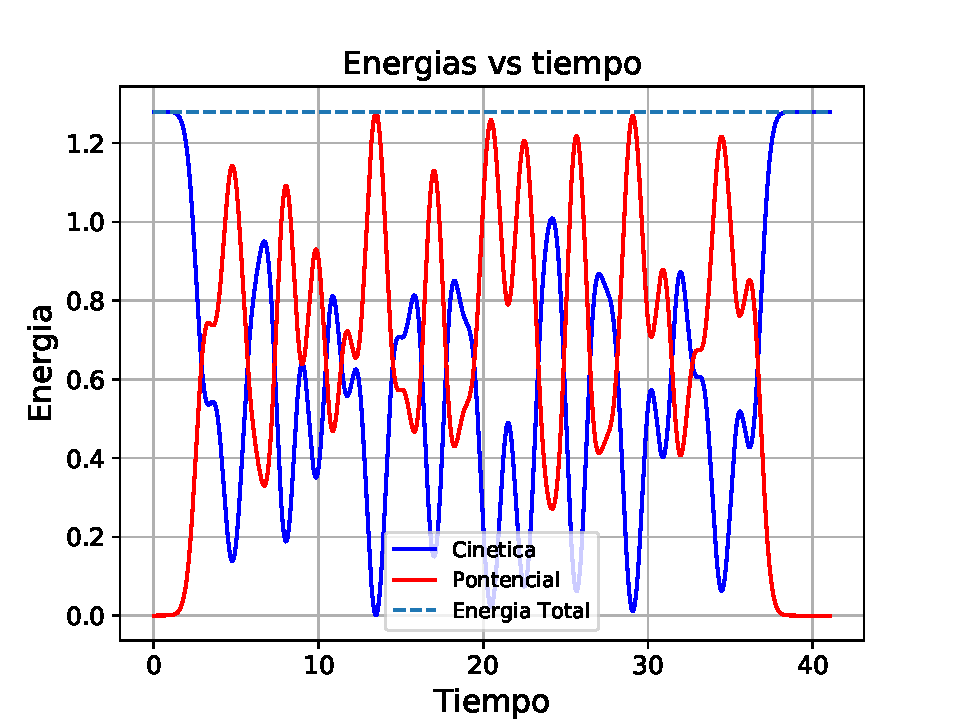
\includegraphics[scale=0.55]{g3.pdf}
\caption{Energias de la trayectoria 1.}
\label{ene}
\end{figure}   
\par 
Debido a que el pozo de potencial se encuentra justo sobre el observador, el punto en x de tiro ($x_{o}$) coincide con el parámetro de impacto $\gamma$ con respecto al centro común de los potenciales; al realizar un lanzamiento con un parámetro de impacto cercano al anterior, con los mismos parámetros y la misma velocidad inicial, se observa en la figura \ref{f3} una trayectoria distinta a la observada en la figura \ref{f1}, lo cual sugiere que el sistema se comporta de manera caótica.
\begin{figure}[H]
\centering 
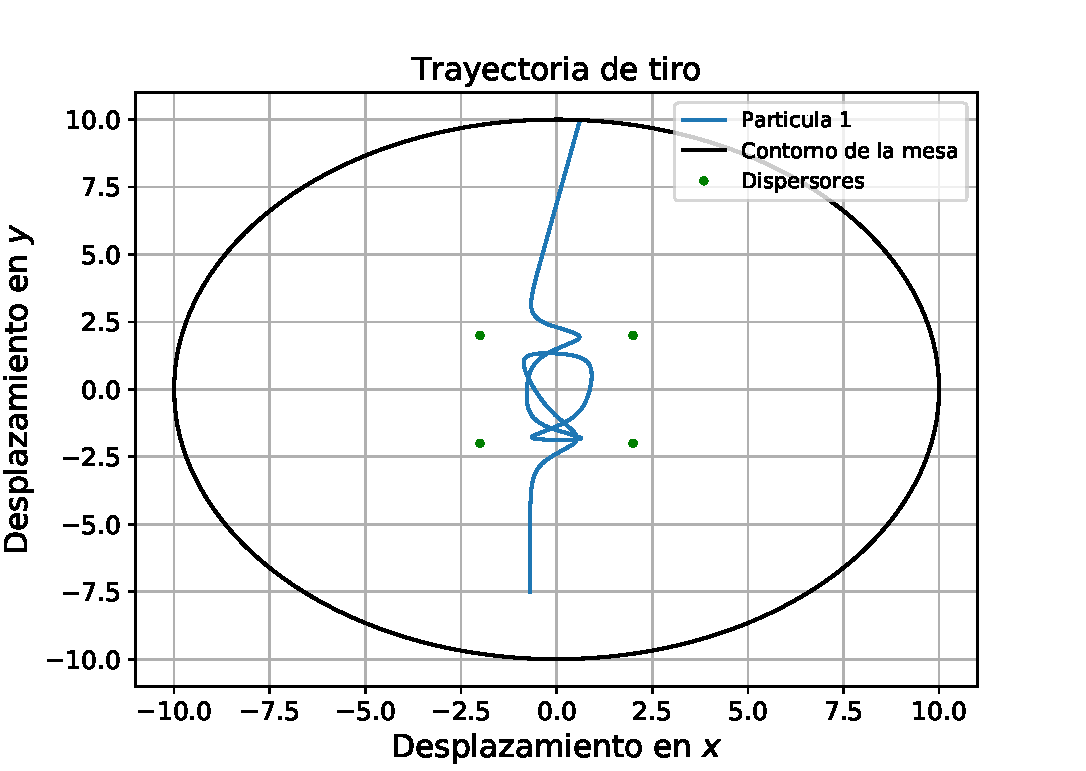
\includegraphics[scale=0.5]{g4.pdf}
\caption{Particula lanzada con las mismas condiciones y parámetros que la trayectoria de la figura 1, pero con $\gamma$=0.69}
\label{f3}
\end{figure}   
\par 
\par 
Con el motivo de estudiar a profundidad ésta problemática, se implemento una función que efectuará dos lanzamientos con las mismas condiciones iniciales, variando solo por un delta el parámetro de impacto $\gamma$, y a partir de los datos de las trayectorias, determinara la separación espacial entre punto y punto de éstas, para cada instante del tiempo. Esto permitió analizar la separación entre las trayectorias en función del tiempo, en pequeños intervalos de tamaño N, a través de un fitting utilizando la función optimize.curve-fit de la librería Scipy, del cual se obtiene los coeficientes de Lyapunov según la ecuación \ref{coef}, para cada intervalo de tamaño N. Ésta función también almacena las distancias con respecto al origen, del punto medio de las posiciones analizadas para cada intervalo, de cada partícula, permitiendo relacionar el coeficiente de Lyapunov con una distancia media al centro de los potenciales.\\
\begin{figure}[H]
\centering 
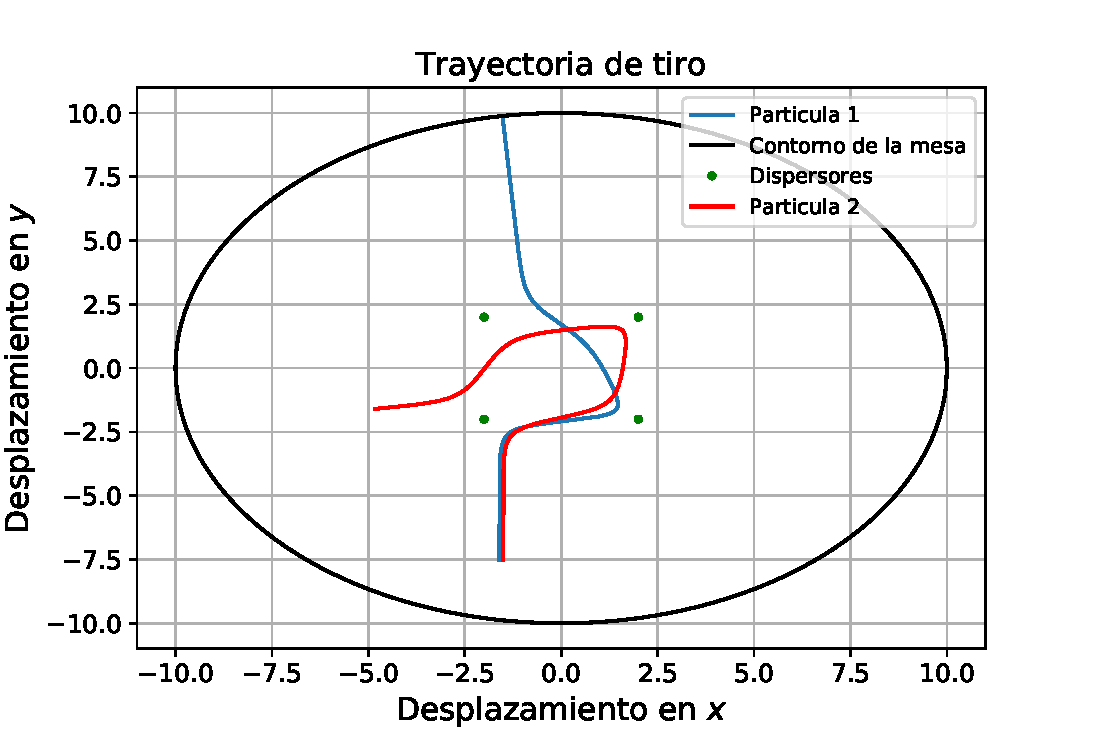
\includegraphics[scale=0.5]{g5.pdf}
\caption{Gráfica de las trayectorias con parámetros=[m: 1, $\alpha: 0$.$5$, $R: 10$ , $A: 3$, $ v_{o}: $2.$3$, $a$: 2], $\gamma=-1.6$ con $\delta_{o}$=$0.01$}
\label{f4}
\end{figure}  
\par 
En la figura \ref{f4} , se observa el lanzamiento de dos partículas con un $\gamma=-1.6$ y un delta de $\delta_{o}=0.01$ ,y en la figura \ref{f5} se observa como varia su separación espacial en el tiempo. 
\begin{figure}[H]
\centering 
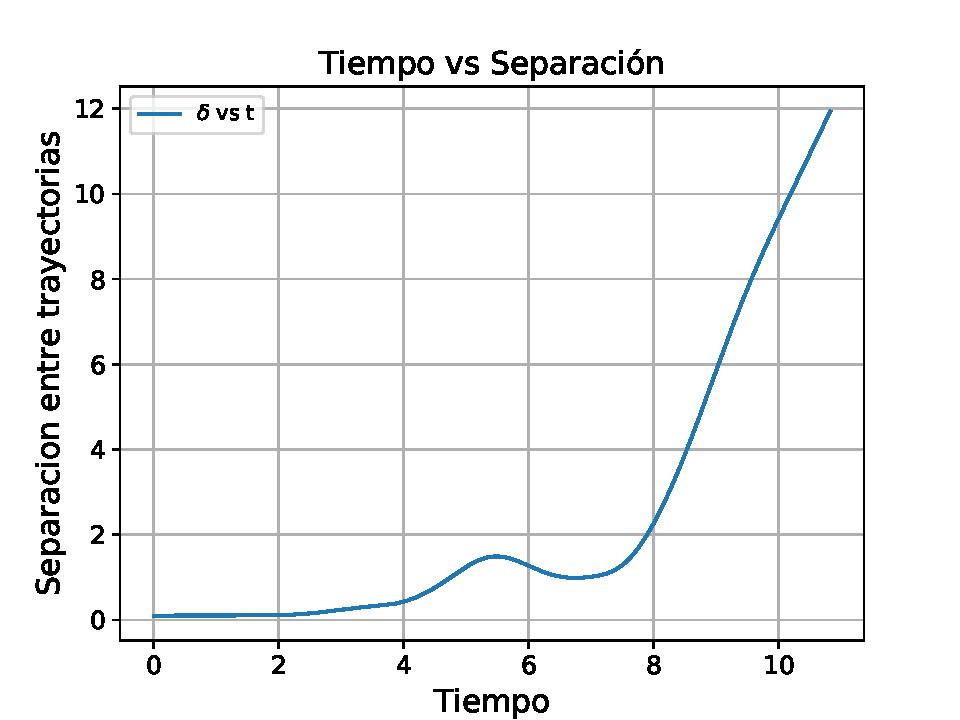
\includegraphics[scale=0.55]{g6.pdf}
\caption{Separación espacial de las trayectorias de la figura \ref{f4}, en función del tiempo.}
\label{f5}
\end{figure}  
\par 
Al realizar el fitting de la gráfica anterior por pequeños intervalos de tamaño $N=30$, se determinaron sus coeficientes de Lyapunov, para el par de trayectorias. Al graficar éstos ($\lambda$) en función de la distancia media al centro de los potenciales de cada partícula, ver figura \ref{f6}, se observa cómo aumenta el valor del coeficiente a medida que las partículas se acerca al centro, encontrando la zona en la que hubo caos, es decir $ \vert \lambda \vert > 1$. Para este par, el caos ocurre cuando las partículas se encuentran entre 1 y 3 unidades de distancia con respecto al centro de los potenciales.\\
\begin{figure}[H]
\centering 
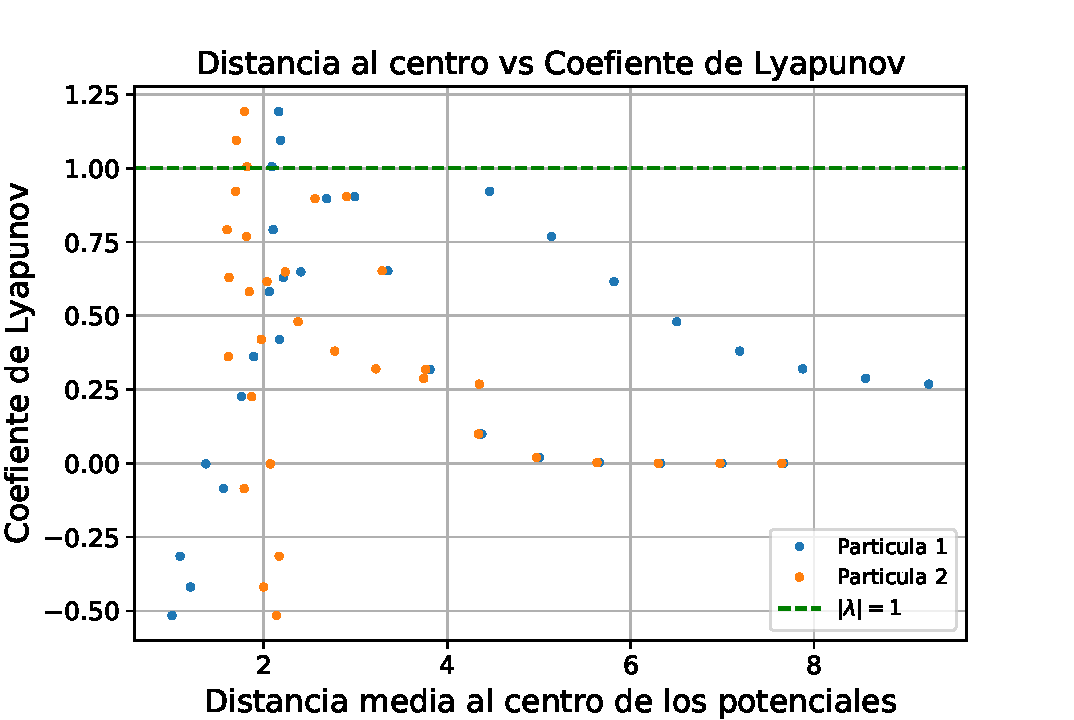
\includegraphics[scale=0.5]{g7.pdf}
\caption{Coeficientes de Lyapuno de las trayectorias de la figura \ref{f4}, en funcion de la distancia media al centro de los potenciales, de cada partícula.}
\label{f6}
\end{figure}
\par 
Con el fin de corroborar a que distancia distancia hubo caos, es decir una separacion abrupta entre las trayectorias, se grafico en la figura \ref{f7}, la separacion entre las trayectorias en función de la distancia con respecto al centro común de los potenciales, de cada partícula. Verificando en este caso, que la zona en la que se separan las trayectorias de manera abrupta, es cuando las partículas se encuentran a una distancia del centro, entre 1 y 3 unidades. 
\begin{figure}[H]
\centering 
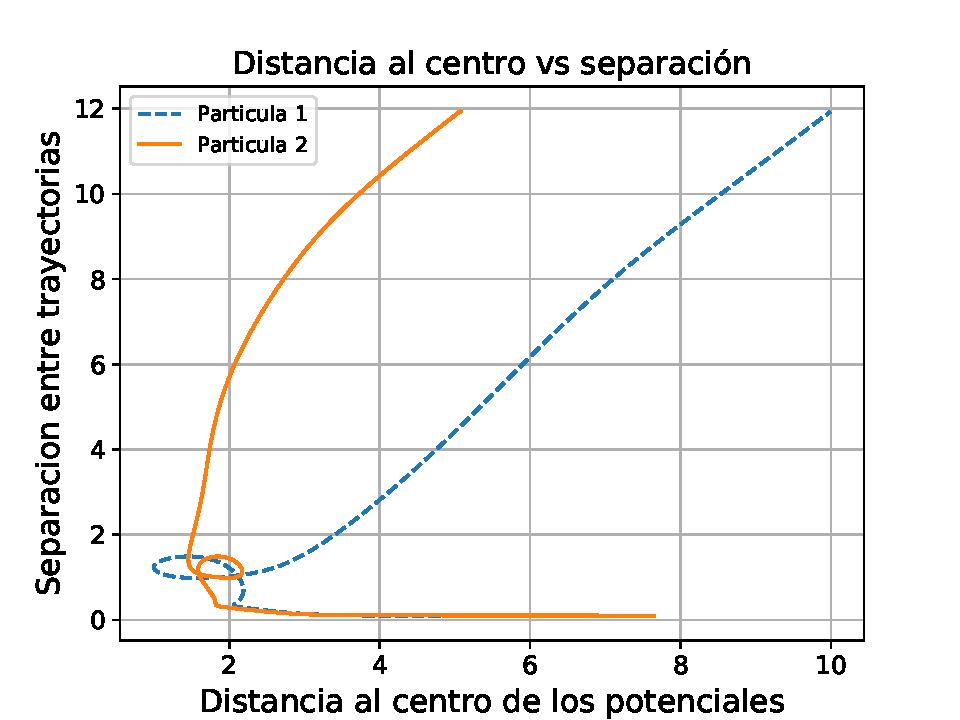
\includegraphics[scale=0.55]{g8.pdf}
\caption{Separación espacial de las trayectorias de la figura \ref{f4}, en funcion de la distancia al centro de los potenciales, de cada partícula.}
\label{f7}
\end{figure}    
\par 
En las figuras \ref{f1}, \ref{f3} y \ref{f4}, se observa que el caos presente en la trayectoria, también depende  del punto en x, desde el cual es lanzada la partícula, es decir el parámetro de impacto. Para comprobar esto, se creo una función que lanzara dos partículas, barriendo desde $\gamma_{i}$ hasta $\gamma_{f}$ el parámetro de impacto, con un delta $\delta_{o}$ ; y almacenara el coeficiente de mayor valor. Permitiendo graficar el valor máximo encontrado del coeficiente de Lyapunov, para cada par de trayectorias en función del parámetro de impacto $\gamma$, como se observa en la figura \ref{f8}.
 
\begin{figure}[h!]
\centering 
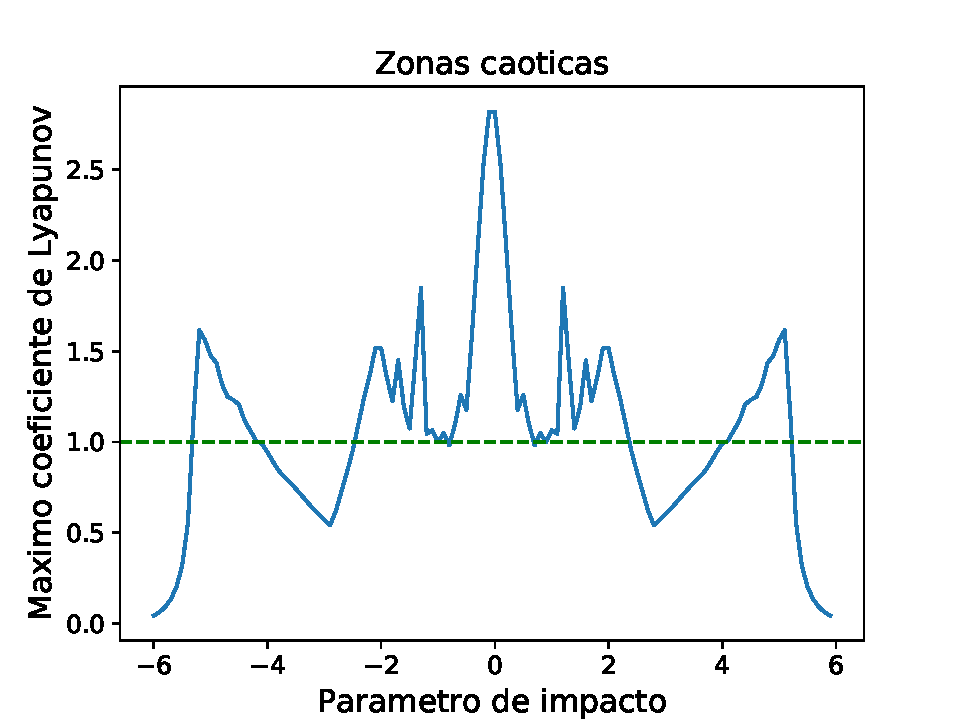
\includegraphics[scale=0.55]{g9.pdf}
\caption{Maximo coeficiente de Lyapunov en funcion del parametro de impacto, con parámetros=[m: 1, $\alpha: 0$.$5$, $R: 10$ , $A: 3$, $ v_{o}: $2.$3$, $a$: 2], $\gamma_{i}=-6$, $\gamma_{f}=6$, $N=30$ y $\delta_{o}=0.01$}
\label{f8}
\end{figure}    
\par 
Én la figura anterior, se aprecia la zona caotica, donde gran mayoria de los pares de lanzamientos presentan al menos un coefiente $\vert \lambda \vert \geq 1$, la cual ésta comprendida cuando el parametro de impacto toma valores aproximados en el intervalo $(-2$.$5$,$2$.$5)$; sin embargo, se observan dos picos a los extremos de la grafica, estos corresponde a la zona del espacio donde la intensidad de un campo puede llegar a tener una diferencia de varios ordenes de magnitud con respecto a otro potencial; ya que la intensidad de los potenciales depende de un exponencial, pequeñas variaciones en el parametro de impacto, implicaria en ésta zona, que una particula experimente una mayor interaccion por parte de los potenciales, con respecto a otra lanzada con parametro de impacto ligeramente mayor; ésto se evidencia, ya que a medida que el parametro de impacto se acerca al origen, sin entrar en la zona caotica, el caos disminuye, debido a que particulas con parametros de impacto cercanos, presentan interacciones similiares con los dispersores.\\
%(arriba) Corregir esta parte decir que para pequeñas vairaciones la partiucla puede o no sentir mas de un potencial 
\par 
La región caotica para cierta configuracion de los potenciales, no solo depende del parametro de impacto, sino tambien de la velocidad con la que son lanzadas las particulas, debido a que entre mayor sea su energia cinetica, menor sera el efecto de desviacion producto de la inetracción con los potenciales sobre la particula. Teniendo lo anterior en consideracion, se realizo el mismo barrido de la figura \ref{f8}, pero lanzando las particulas con una velocidad inicial $v_{o}=3.6$, con el proposito de evidenciar ésta dependencia, como se observa en la figura \ref{caoss}, donde es evidente una reduccion en el tamaño de la zona caotica. 
\begin{figure}[h!]
\centering 
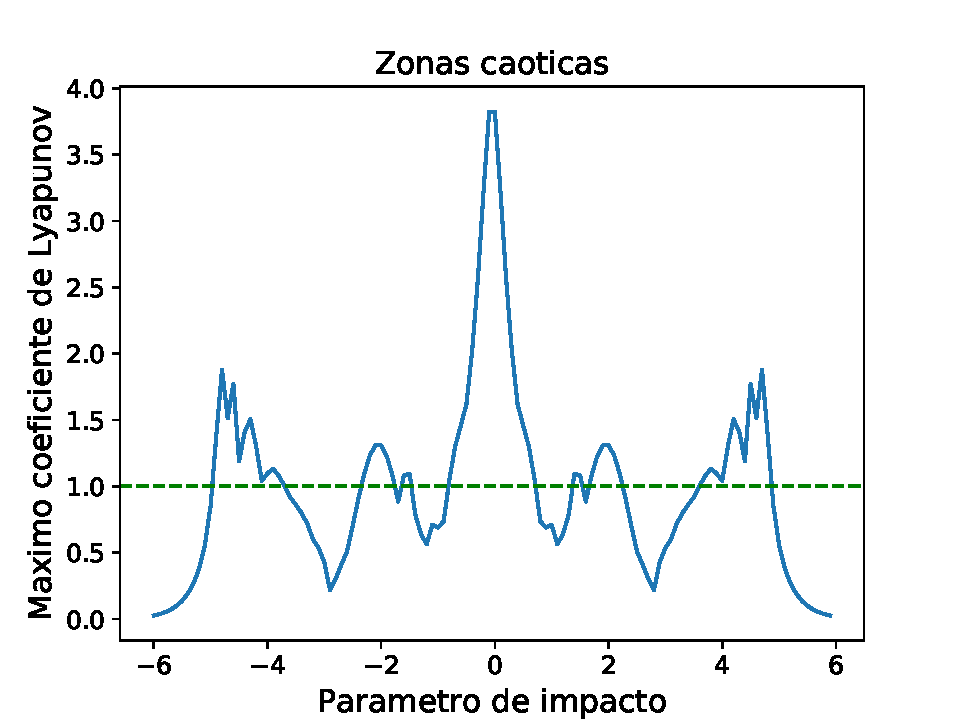
\includegraphics[scale=0.55]{g10.pdf}
\caption{Maximo coeficiente de Lyapunov en funcion del parametro de impacto, con parámetros=[m: 1, $\alpha: 0$.$5$, $R: 10$ , $A: 3$, $ v_{o}: $3.$6$, $a$: 2], $\gamma_{i}=-6$, $\gamma_{f}=6$ y $\delta_{o}=0.01$}
\label{caoss}
\end{figure}
\par 
Cómo se ha observado, el punto desde el cual se lanza una partícula influye en la manera como es desviada su trayectoria (ángulo de salida), por lo cual también se ve afectado el punto en el cual impacta con la pared de la mesa, es decir su ángulo de impacto. Para la identificación de los ángulos de salida e impacto, se tomaron los ángulos con respecto a la vertical desde $0$ hasta $180$ grados, con la convención de ángulos positivos en el sentido contrario a las manecillas del reloj. Determinando el ángulo de salida ($\theta_{out}$) a través de la expresión:
$$\theta_{out}=\arctan(v_{y_{f}}/v_{x_{f}}) \pm \dfrac{\pi}{2}$$
\par 
Donde $v_{y_{f}}$ y $v_{x_{f}}$ son las componentes del vector velocidad de la partícula al momento de impactar con el contorno de la mesa, y el signo de $\dfrac{\pi}{2}$ depende del cuadrante donde se encuentre el vector velocidad; siendo positivo para los cuadrantes 2 y 3, es decir $(-x,y)$ y $(-x,-y)$ respectivamente, y negativo para los cuadrantes 1 $(x,y)$ y 4 $(x,-y)$. La determinación del ángulo de impacto es similar a la del ángulo de salida, sin embargo, éste se encuentra mediante la expresión:
$$\theta_{impact}=\arctan(x_{y_{f}}/x_{x_{f}}) \pm \dfrac{\pi}{2}$$
\par 
Donde $x_{y_{f}}$ y $x_{x_{f}}$ son las componentes del vector posición de la partícula al momento de impactar con el contorno de la mesa, y el signo de $\dfrac{\pi}{2}$ depende del cuadrante donde se encuentre el vector posición.\\
\par 
Teniendo lo anterior en consideración, se construyo una función que barriera los parámetros de impacto en un intervalo $[\gamma_{i},\gamma_{f}]$ a un paso de $\delta_{o}$, y para cada elemento de éste, lanzara una partícula y almacenara sus ángulos de salida e impacto. En la figura \ref{f9}, se visualiza el ángulo de salida en función del parámetro de impacto, es decir la manera o el grado en el que son dispersadas las partículas en función del parámetro de impacto, para un set de parametros especifico.\\
  
\begin{figure}[H]
\centering 
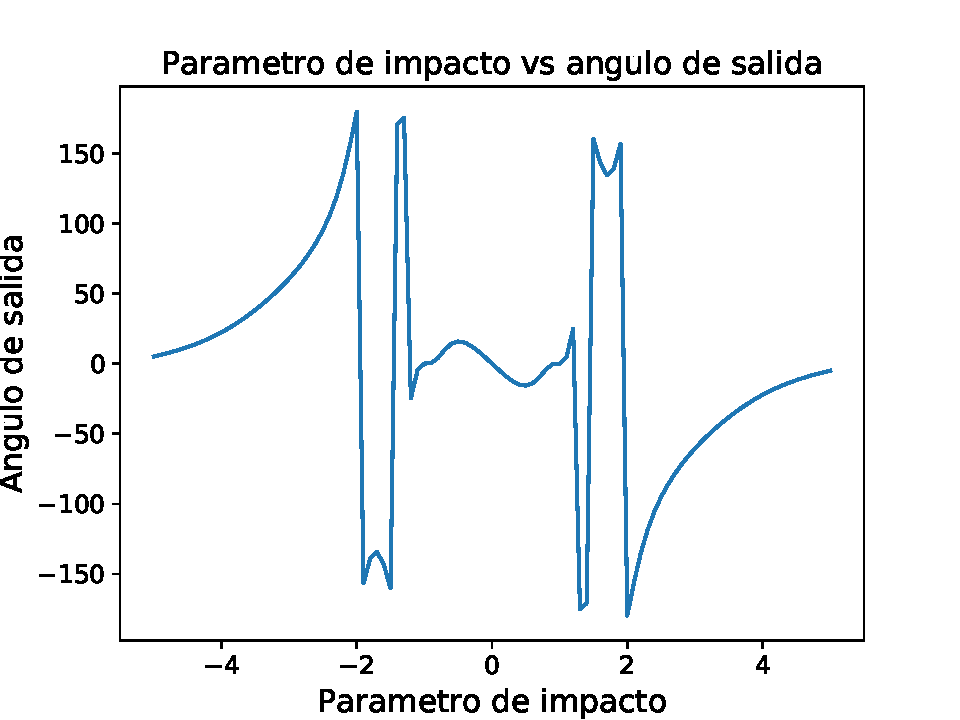
\includegraphics[scale=0.59]{g11.pdf}
\caption{Angulo de salida en función del parámetro de impacto, con parámetros=[m: 1, $\alpha: 0$.$5$, $R: 10$ , $A: 3$, $ v_{o}: $2, $a$: 2], $\gamma_{i}=-5$, $\gamma_{f}=5$ y $\delta_{o}=0.01$}
\label{f9}
\end{figure}    
\par 
La manera como son dispersadas las partículas depende de las características de los dispersores ($A$ y $\alpha$), sin embargo, también depende de la energía con la que son lanzadas las partículas, puesto que entre mayor sea su energía cinética, menor sera el efecto de desviación producto de la interacción con los potenciales sobre la partícula. Esto queda en evidencia en la figura \ref{f10}, donde se realiza el mismo barrido que en la figura \ref{f9}, pero con una rapidez inicial de $v_{o}=2 \sqrt{2}$, es decir las partículas son lanzadas con el doble de energía cinética; y se observa como disminuyen los ángulos, es decir el grado, con el que son dispersadas las partículas.\\  
  
\begin{figure}[H]
\centering 
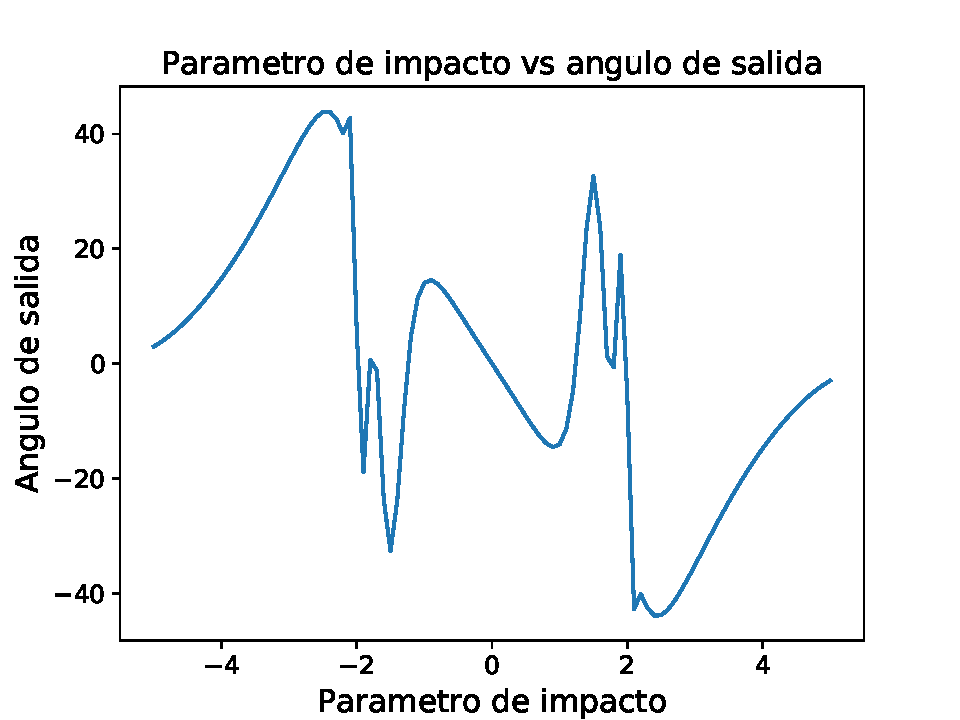
\includegraphics[scale=0.55]{g12.pdf}
\caption{Ángulo de salida en función del parámetro de impacto, con parámetros=[m: 1, $\alpha: 0$.$5$, $R: 10$ , $A: 3$, $ v_{o}: $2$\sqrt{2}$, $a$: 2], $\gamma_{i}=-5$, $\gamma_{f}=5$ y $\delta_{o}=0.01$}
\label{f10}
\end{figure}
 
\par 
Debido a que no todas las partículas son desviadas de igual manera, existen áreas en el contorno de la mesa, en las que ocurre una mayor cantidad de impactos que en otras. Con la intención de determinar la sección eficaz de impacto$^{[2]}$, se realizo un histograma de los ángulos de salida (figura \ref{f11}), para los lanzamientos de la figura \ref{f9}. En la que se visualiza la distribución de impacto sobre el contorno de la mesa, donde la región eficaz se encuentra entre las cercanías al ángulo cero. 
\begin{figure}[H]
\centering 
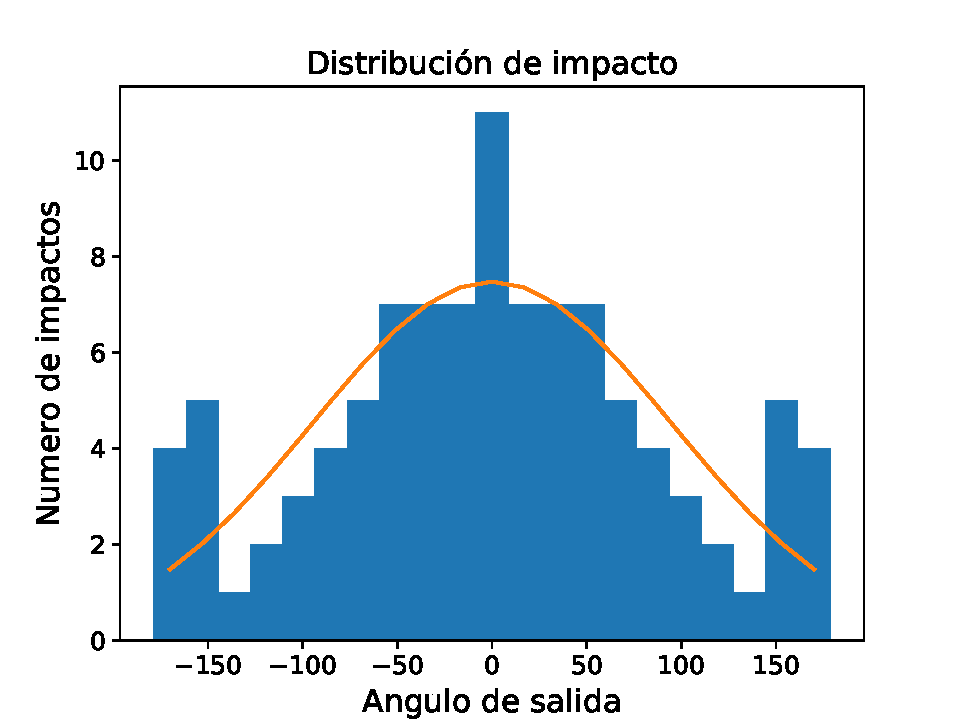
\includegraphics[scale=0.55]{g13.pdf}
\caption{Distribución de impacto, con parámetros=[m: 1, $\alpha: 0$.$5$, $R: 10$ , $A: 3$, $ v_{o}: $2, $a$: 2], $\gamma_{i}=-5$, $\gamma_{f}=5$ , $\delta_{o}=0.01$ y $\overline{x}=0.0016^{\circ} $}
\label{f11}
\end{figure}
\par 
Sin embargo, de igual manera a los análisis anteriores, al variar la energía con la que son lanzadas las partículas, se produce un cambio en la manera como se comporta el sistema como un global; en éste caso al lanzar las partículas con la mitad de la energía que en la figura \ref{f11}, es decir $v_{o}=\sqrt{2}/2$, se observa en la figura \ref{ul}, cómo las partículas son desviadas a los costados y principalmente en sentido contrario, puesto que son repelidas antes de entrar en el medio de los potenciales, ocasionando que la sección eficaz se encuentre en una posición opuesta de la mesa, con respecto a la sección eficaz de la figura \ref{f11}.  
\begin{figure}[H]
\centering 
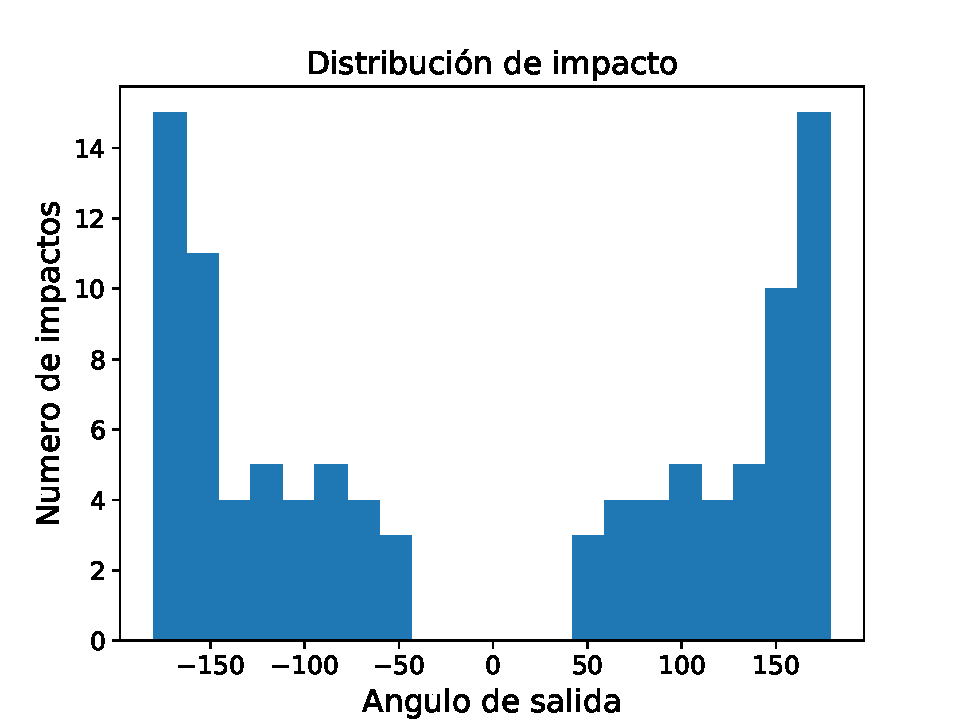
\includegraphics[scale=0.55]{g14.pdf}
\caption{Distribución de impacto, con parámetros=[m: 1, $\alpha: 0$.$5$, $R: 10$ , $A: 3$, $ v_{o}: \sqrt{2}/2$, $a$: 2], $\gamma_{i}=-5$, $\gamma_{f}=5$ y $\delta_{o}=0.01$}
\label{ul}
\end{figure}

\section*{\normalsize{CONCLUSIÓN}}
Mediante las herramientas computacionales hechas en Python, y el runge kutta de orden 4, se pudo estudiar y modelar un sistema físico del lanzamiento bidimensional de una partícula, en un entorno cerrado circular con cuatro dispersores situados alrededor del centro; se comprobó mediante los coeficientes de Lyapunov que el sistema presenta caos en la región comprendida aproximadamente en el intervalo $(-2$.$5$,$2$.$5)$ para un set de parámetros con [$m: 1$, $\alpha: 0$.$5$, $R: 10$ , $A: 3$, $ v_{o}: 2$.$3$, $a$: 2, $\gamma_{i}=-6$, $\gamma_{f}=6$], y se observo que la región caótica cambia al variar la energía inicial del sistema; también se comprobó que la energía del sistema se conserva, además, se observo como depende el grado de dispersión causado por los potenciales sobre la partícula (el cual es simétrico), del parámetro de impacto y de la energía inicial de lanzamiento, para un set de parámetros específicos. De manera similar se obtuvo la distribución de impacto sobre el contorno de la mesa para un set de parametros con [$m:1$, $\alpha: 0$.$5$, $R: 10$ , $A: 3$, $ v_{o}:2$, $a$: 2], permitiendo determinar la sección eficaz, la cual se encuentra alrededor del ángulo de impacto $0^{\circ}$ , y observar que ésta varia al cambiar la energía inicial de lanzamiento.
\section*{Referencias} 
\begin{itemize} 
\item[[ 1]] Notas de clase-Física computacional 1. Prof. Juan Carlos Cardona, Doctor en ciencias físicas. Docente del programa de Física, Universidad del Atlántico, Barranquilla-Colombia. 

\item[[ 2]] Goldstein,H. Mecánica clásica. Reverte,1987. Ediccion 2017.

\item[[ 3]] Regiones de comportamiento atípico en billares caóticos. In memoriam M. en C. Jorge Alejandro Hernández Tahuilán. 

\item[[ 4]] Revista de la Academia Mexicana de Ciencias. Abril-Junio 2011. Volumen 62 número 2.
\end{itemize}

\end{document}
